\section{Ristrutturazione schema E-R}
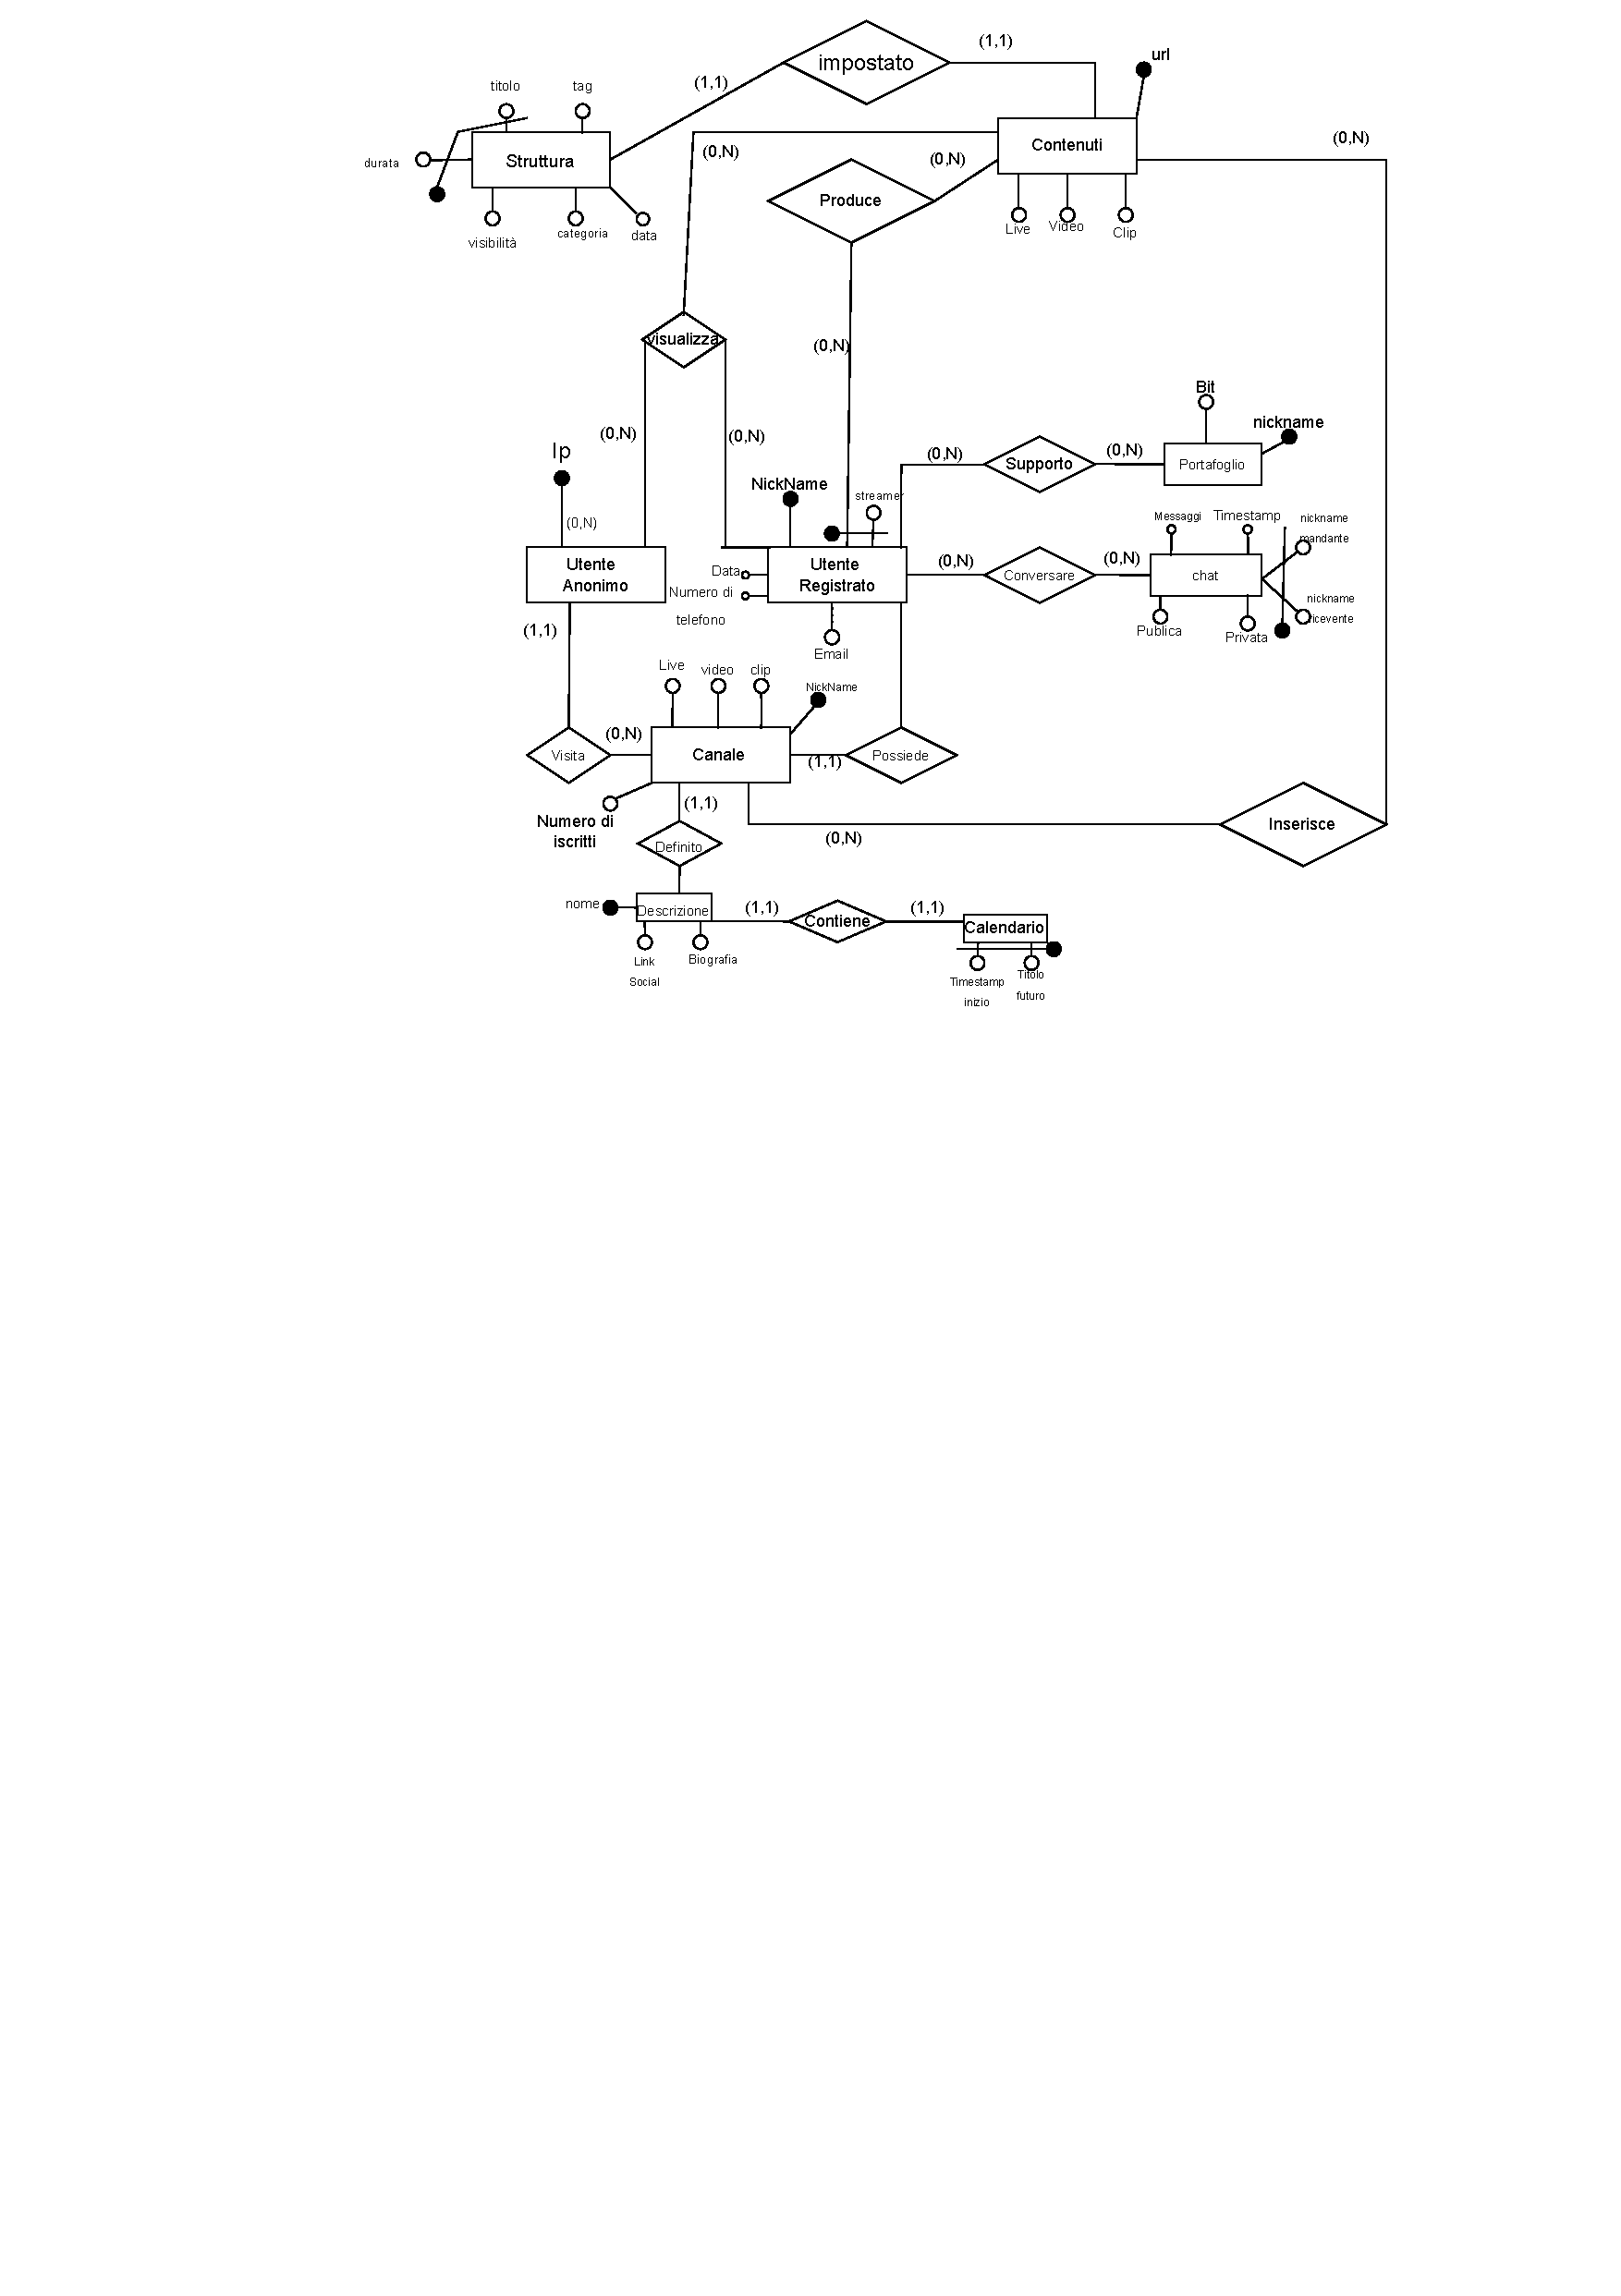
\includegraphics[width=\textwidth]{resources/e_r-ridotto.pdf}

\section{Analisi delle Ridondanze}
Le ridondanze trovate sono le seguenti:
\begin{enumerate}
    \item Il nome del canale è derivabile dal nickname dell'utente registrato
    \item Gli attributi dell'entità \textit{Contenuti} sono ricavabili dall' entità \textit{Canale}
    \item I messaggi inviati dagli utenti non hanno un identificativo che indica se un messaggio è pubblico o privato, quindi se un messaggio si trova all'interno di una
          chat pubblica o privata esso sarà comunque un messaggio quindi è ricavabile dall'entità chat. 
\end{enumerate}
\subsubsection{Ridondanza dei messaggi pubblici/privati}
\begin{itemize}
    \item La presenza di ridondanza nella gestione dei messaggi in chat comporta un aumento significativo
     della quantità di memoria. L'attributo "Chat" memorizza messaggi indipendentemente dalla loro natura
      pubblica o privata, poiché la distinzione tra i due è rilevante solo per il tipo di messaggio. 
      Senza ridondanza, i messaggi sono gestiti separatamente in chat individuali, ciascuna con una propria 
      quantità di messaggi da elaborare, evitando un raggruppamento in una sezione comune di memoria. 

\end{itemize}

Si ipotizzano 1.000.000.000 di messaggi scambiati, con la ridondanza un messaggio non viene distinto tra pubblico e privato, quindi viene contato doppio
\subsubsection{Analisi con ridondanza}
Tempo impiegato : $\frac{2.000.000.000 messaggi * 1 ms}{messaggi *2 }$\footnote{i messaggi sono il doppio di quelli effettivi in quanto non vengono distintio, perazioni di read and write} $\simeq 32$ minuti per salvare tutti i messaggi. \\
Spazio: Si ipotizza 100 kb a messaggio, considerando la mole prevista di messaggi $\simeq 190$ GB di spazio utilizzato. 
\small
\begin{longtable}{|l|c|c|p{6.2cm}|}
  \hline \textbf{Concetto} & \textbf{Tipo} & \textbf{Accessi} & \textbf{Tipo} \\\hline
  \endfirsthead

  \hline \textbf{Concetto} & \textbf{Tipo} & \textbf{Accessi} & \textbf{Tipo} \\\hline
  \endhead

  \hline \multicolumn{4}{|r|}{\textit{Continua alla pagina successiva}}
  \endfoot
    Utente Registrato & R/W & Conversare & 2.000.000.000 \\\hline
  \endlastfoot


\end{longtable}
\normalsize
\newpage
\subsubsection{Analisi senza ridondanza}
Tempo impiegato : $\frac{1.000.000.000 * 0.5 ms}{messaggi * 2}$ \footnote{operazioni di read and write} $\simeq 16$ minuti per salvare tutti \\
Spazio: Si ipotizza 100 kb a messaggio, quindi in termini di spazio totali $\simeq 90$ GB occupati.  
%Inserire motivazioni di questa scelta + aggiunta accessi e entità ( messaggio privato || messaggio pubblico )
%Abbiamo che aumentiamo di N gli accessi per messaggi privati e K accessi per messaggi pubblici 
\newline
\small
\begin{longtable}{ |l|c|c|p{6.2cm}|}
  \hline \textbf{Concetto} & \textbf{Tipo} & \textbf{Accessi} & \textbf{Tipo} \\\hline
  \endfirsthead

  \hline \textbf{Concetto} & \textbf{Tipo} & \textbf{Accessi} & \textbf{Tipo} \\\hline
  \endhead

  \hline \multicolumn{4}{|r|}{\textit{Continua alla pagina successiva}}
  \endfoot

    Utente Registrato& R/W & Conversare & 1.000.000.000 \\\hline
  \endlastfoot

\end{longtable}
\normalsize
\section{Eliminazioni delle Generalizzazioni}
Le generalizzazioni presenti nello schema E-R sono:
\begin{enumerate}
    \item \textbf{Utente}: È una generalizzazione totale tra le entità \textit{Utente registrato} e \textit{Utente anonimo}, poichè o si è registrati alla piattaforma o si è anonimi
    \item \textbf{Streamer e Streamer-Spettatore}: È una generalizzazione parziale tra le entità \textit{Streamer} e \textit{Streamer-Spettatore}, in quanto l'utente registrato si ritrova a svolgere il ruolo o di streamer o di spettatore, ma sempre essendo uno streamer  
    \item \textbf{Spettatore - Utente Anonimo}: È una generalizzazione sovrapposta, poiché l'utente anonimo può essere solo spettatore
    \item \textbf{Chat}: È una generalizzazione totale tra le entità \textit{Chat privata} e \textit{Chat pubblica}. Perché l'entià chat si divide in due sottoinsiemi, ovvero chat pubblica e chat privata.
\end{enumerate} 
\section{Partizionamento/Accorpamento di entità e associazioni}
Si è deciso di accorpare l'entità chat, così indica in maniera più coincisa che un utente registrato può comunicare in maniera pubblica o privata
\begin{figure}[ht]
    \centering
    \begin{minipage}{.45\textwidth}
        \centering
        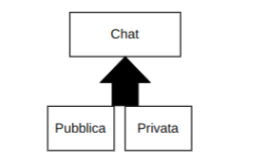
\includegraphics[width=0.9\linewidth]{resources/chat_revised.png}
        \caption{Entità chat dopo l'accorpamento}
        \label{Entità chat dopo l'accorpamento}
    \end{minipage}%
    \begin{minipage}{.5\textwidth}
        \centering
        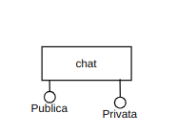
\includegraphics[width=0.9\linewidth]{resources/chat.png}
        \caption{Entità chat prima dell'accorpamento}
        \label{Entità chat prima dell'accorpamento}
    \end{minipage}
\end{figure}

\section{Business rules dell'E-R ristrutturato }
\begin{itemize}
    \item Gli attributi live, video, clip presenti nell'entità \textbf{canale} indicano un contenuto finito e caricato al suo interno.
    \item Gli attributi live, video, clip presenti sull'entitá \textbf{contenuti} indicano un contenuto che ancora o è in fase di produzione o è un prodotto finito ma non caricato sul canale del proprietario. 
    \item Gli utenti anonimi non possono supportare gli streamer. 
    \item Gli streamer sono utenti registrati che caricano  o trasmettono contenuti. 
    \item Ogni utente registrato ha un nickname. 
    \item Il nickname scelto dall'utente registrato sarà anche il nome del canale. 
    \item Ogni canale ha una Descrizione. 
    \item Le live sono contenuti in tempo reale.
    \item I video sono live già concluse. 
    \item Le clip sono brevi estratti di video. 
    \item Un utente anonimo non può conversare con altri utenti.
    \item Un utente anonimo non possiede un canale. 
\end{itemize}
